% You should title the file with a .tex extension (hw1.tex, for example)
\documentclass[11pt]{article}

\usepackage{hyperref}
\usepackage{amsmath}
\usepackage{mathtools}
\usepackage{amssymb}
\usepackage{wrapfig}
\usepackage{fancyhdr}
\usepackage{tikz-qtree}
\usepackage{tikz-qtree-compat}
\usepackage[normalem]{ulem}
\usepackage{tikz}
\usepackage{systeme}
\usepackage{graphicx}
\DeclareMathOperator*{\argmin}{argmin}
\DeclareMathOperator*{\argmax}{argmax}
\usepackage{bm}

\oddsidemargin0cm
\topmargin-2cm     %I recommend adding these three lines to increase the 
\textwidth16.5cm   %amount of usable space on the page (and save trees)
\textheight23.5cm  

\newcommand{\question}[2] {\vspace{.25in} \hrule\vspace{0.5em}
\noindent{\bf #1: #2} \vspace{0.5em}
\hrule \vspace{.10in}}
\renewcommand{\part}[1] {\vspace{.10in} {\bf (#1)}}

\newcommand{\myname}{Sean Bittner}
\newcommand{\myandrew}{srb2201@columbia.edu}
\newcommand{\myhwnum}{12}

\setlength{\parindent}{0pt}
\setlength{\parskip}{5pt plus 1pt}
 
\DeclarePairedDelimiter\abs{\lvert}{\rvert}%
 %
\pagestyle{fancyplain}
\rhead{\fancyplain{}{\myname\\ \myandrew}}

\begin{document}

\medskip                        % Skip a "medium" amount of space
                                % (latex determines what medium is)
                                % Also try: \bigskip, \littleskip

\thispagestyle{plain}
\begin{center}                  % Center the following lines
{\Large Draft of new V1 section} \\
Sean Bittner, Agostina Palmigiano \\
November 24, 2020 \\
\end{center}

\section{Exploratory analysis of V1 with EPI produces a novel theory}\label{results_V1}
Dynamical models of excitatory (E) and inhibitory (I) populations with supralinear input-output function have succeeded in explaining a host of experimentally documented phenomena.
In a regime characterized by inhibitory stabilization of strong recurrent excitation, these models give rise to paradoxical responses \cite{tsodyks1997paradoxical}, selective amplification  \cite{goldman2009memory, murphy2009balanced}, surround suppression \cite{ozeki2009inhibitory} and normalization \cite{rubin2015stabilized}. 
Despite their strong predictive power, E-I circuit models rely on the assumption that inhibition can be studied as an indivisible unit. 
However, experimental evidence shows that inhibition is composed of distinct elements -- parvalbumin (P), somatostatin (S), VIP (V) --
composing 80\% of GABAergic interneurons in V1 \cite{markram2004interneurons, rudy2011three, tremblay2016}, and that these inhibitory cell types follow specific connectivity patterns (Fig. \ref{fig:Fig3}A) \cite{pfeffer2013inhibition}.
Recent theoretical advances \cite{litwin2016inhibitory, GarciaDelMolino2017, Chen2019},  have only started to address the consequences of this multiplicity in the dynamics of V1, strongly relying on linear theoretical tools. 
Here, we use EPI to elucidate the mechanisms of neuron-type stability in V1 at different levels of contrast.

We considered the contrast responses of a nonlinear dynamical V1 circuit model (Fig. \ref{fig:Fig3}A) with a state comprised of each neuron-type population's rate $\mathbf{x} = \left[x_E, x_P , x_S, x_V \right]^\top$.
Each population receives recurrent input $W \mathbf{x}$ from synaptic projections of effective connectivity $W$ and an external input $\mathbf{h}$, which determine the population rate via nonlinearity $f_r = \left[\right]^2_+$ (see Section \ref{methods_V1}).
The deterministic circuit model evolves form an initial condition $\mathbf{x}(0)$ to a steady-state solution (Fig. \ref{fig:Fig3}B, solid).
When slow noise $\mathbf{\epsilon}$ is introduced, circuit activity fluctuates around this solution (Fig. \ref{fig:Fig3}B dashed), and the model is then a stochastic stabilized supralinear network (SSSN) \cite{hennequin2018dynamical} 
\begin{equation}
    \tau \frac{d\mathbf{x}}{dt} = -\mathbf{x} +f_r(W\mathbf{x} + \mathbf{h})
\end{equation}
At full contrast, input to the E- and P-populations increases 
\begin{equation}
\mathbf{h} = \mathbf{h}_b + c\mathbf{h}_c,
\end{equation}
changing the steady state solution (and fluctuations thereabout)  (Fig. \ref{fig:Fig3}C).
In this analysis, we fixed $W$,$\mathbf{h}_b$, and $\mathbf{h}_c$, which have been fit to contrast responses in mouse V1 using the deterministic model (TODO cite, see Section \ref{methods_V1}).
As contrast changes, so does the degree of stochastic variability of each neuron-type (Fig. \ref{fig:Fig3}D).
Moreover, the circuit transitions into an inhibition-stabilized network (ISN) ($\gamma(\mathbf{x}; \mathbf{z}) < 0$) with increasing contrast (Fig. \ref{fig:Fig3}D inset).
While the ISN-regime and its effects are understood well in E-I networks, its role in this SSSN with inhibitory multiplicity has not been explored.

To study the influence of circuit input on stabilization mechanisms in this stochastic model, we asked what changes in circuit input $d\mathbf{h}$ have little effect on the responses of each neuron-type.
\begin{equation}
\mathbf{z} = \begin{bmatrix} dh_E & dh_P & dh_S & dh_V \end{bmatrix}^{\top}.
\end{equation}
To formulate ``fluctuation constraints" for population $\alpha$  at contrast level $c$ as an emergent property in this stochastic model, we prescribed that the mean change in activity with $dh_\alpha$ is 0 and the variance over both EPI posterior and model stochasticity is a small amount
\begin{equation}\label{eq:EP}
\begin{split}
\mathcal{X}(\alpha, c) ~~:~~  \mathbb{E}_{\mathbf{z}}\begin{bmatrix} dx_\alpha(\mathbf{x}; \mathbf{z},c) \end{bmatrix}  &~~=~~  0  ~~\triangleq~~ \mu  \\ 
\text{Var}_{\mathbf{z}}\begin{bmatrix} dx_\alpha(\mathbf{x}; \mathbf{z},c) \end{bmatrix}  &~~=~~  \begin{bmatrix} 0.05^2 \end{bmatrix} ~~\triangleq~~ \sigma^2 .
\end{split}
\end{equation}
By conditioning on this emergent property, we constrained stochastic fluctuations of circuit models sampled from the EPI posterior to be unbiased and vary to a fixed extent from the steady state solution at $d\mathbf{h}=\mathbf{0}$.

Visualization of the resulting $q_{\bm{\theta}}(\mathbf{z} \mid \mathcal{X}(\alpha, c))$ shows that the EPI posteriors largely agree with sets of parameters obtained using ABC (Fig. \ref{fig:SX1}).
Focusing our attention on $P$-fluctuation constraints at 0\% and 100\% contrast ($\mathcal{X}(P, 0\%)$ and $\mathcal{X}(P, 100\%)$, respectively), we gain insight about how $d\mathbf{h}$ governs mechanisms of stability.  
At 0\% contrast, the SSSN is not inhibition-stabilized, and only local perturbations of positive $dh_E$ and negative $dh_P$ place the circuit in the ISN regime, while $P$-population fluctuations are kept near the 0\% contrast level (Fig. \ref{fig:Fig3}E).
At 100\% contrast, where $h_E$ and $h_P$ are much greater, the SSSN is inhibition-stabilized, and $q_\theta(z \mid \mathcal{X}(P, 100\%)$ reveals distinct patterns of $d\mathbf{h}$ that obey the $P$-fluctuation constraint (Fig. \ref{fig:Fig3}F).
As $dh_V$ decreases, either $dh_P$ and $dh_S$ must increase or decrease together.  When $dh_P$ and $dh_S$ increase together, the circuit leaves the ISN regime, and when they are decreased, the strength of inhibition stabilization grows.
The pattern in $d\mathbf{h}$ producing transitions out of the ISN regime is unapparent when running traditional ABC, even when SSSN noise is reduced to a negligible order of magnitude (Fig. \ref{fig:SX2}).

\clearpage
\begin{figure}[h]
\caption{\small \textbf{A}.  Four-population model of primary visual cortex with excitatory (black), parvalbumin (blue), somatostatin (red), and VIP (green) neurons.   Some neuron-types largely do not form synaptic projections to others  (excitatory and inhibitory projections filled and unfilled, respectively).
\textbf{B}. V1 circuit model simulations at 0\% contrast without (SSN, solid) and with (SSSN, solid) slow noise.
\textbf{C}. Simulations at 100\% contrast.
\textbf{D}. Average responses of the SSSN for all contrasts.  Error bars show the standard deviation of stochastic fluctuations.
\textbf{E}. EPI posterior conditioned on P-fluctuation constraints at 0\% contrast.
Parameter samples are colored by their ISN coefficient.
Bottom-left inset is the posterior predictive distribution of $dx_P$.
\textbf{F}. Same as E. at 100\% contrast.
 }\label{fig:Fig3}
\begin{center}
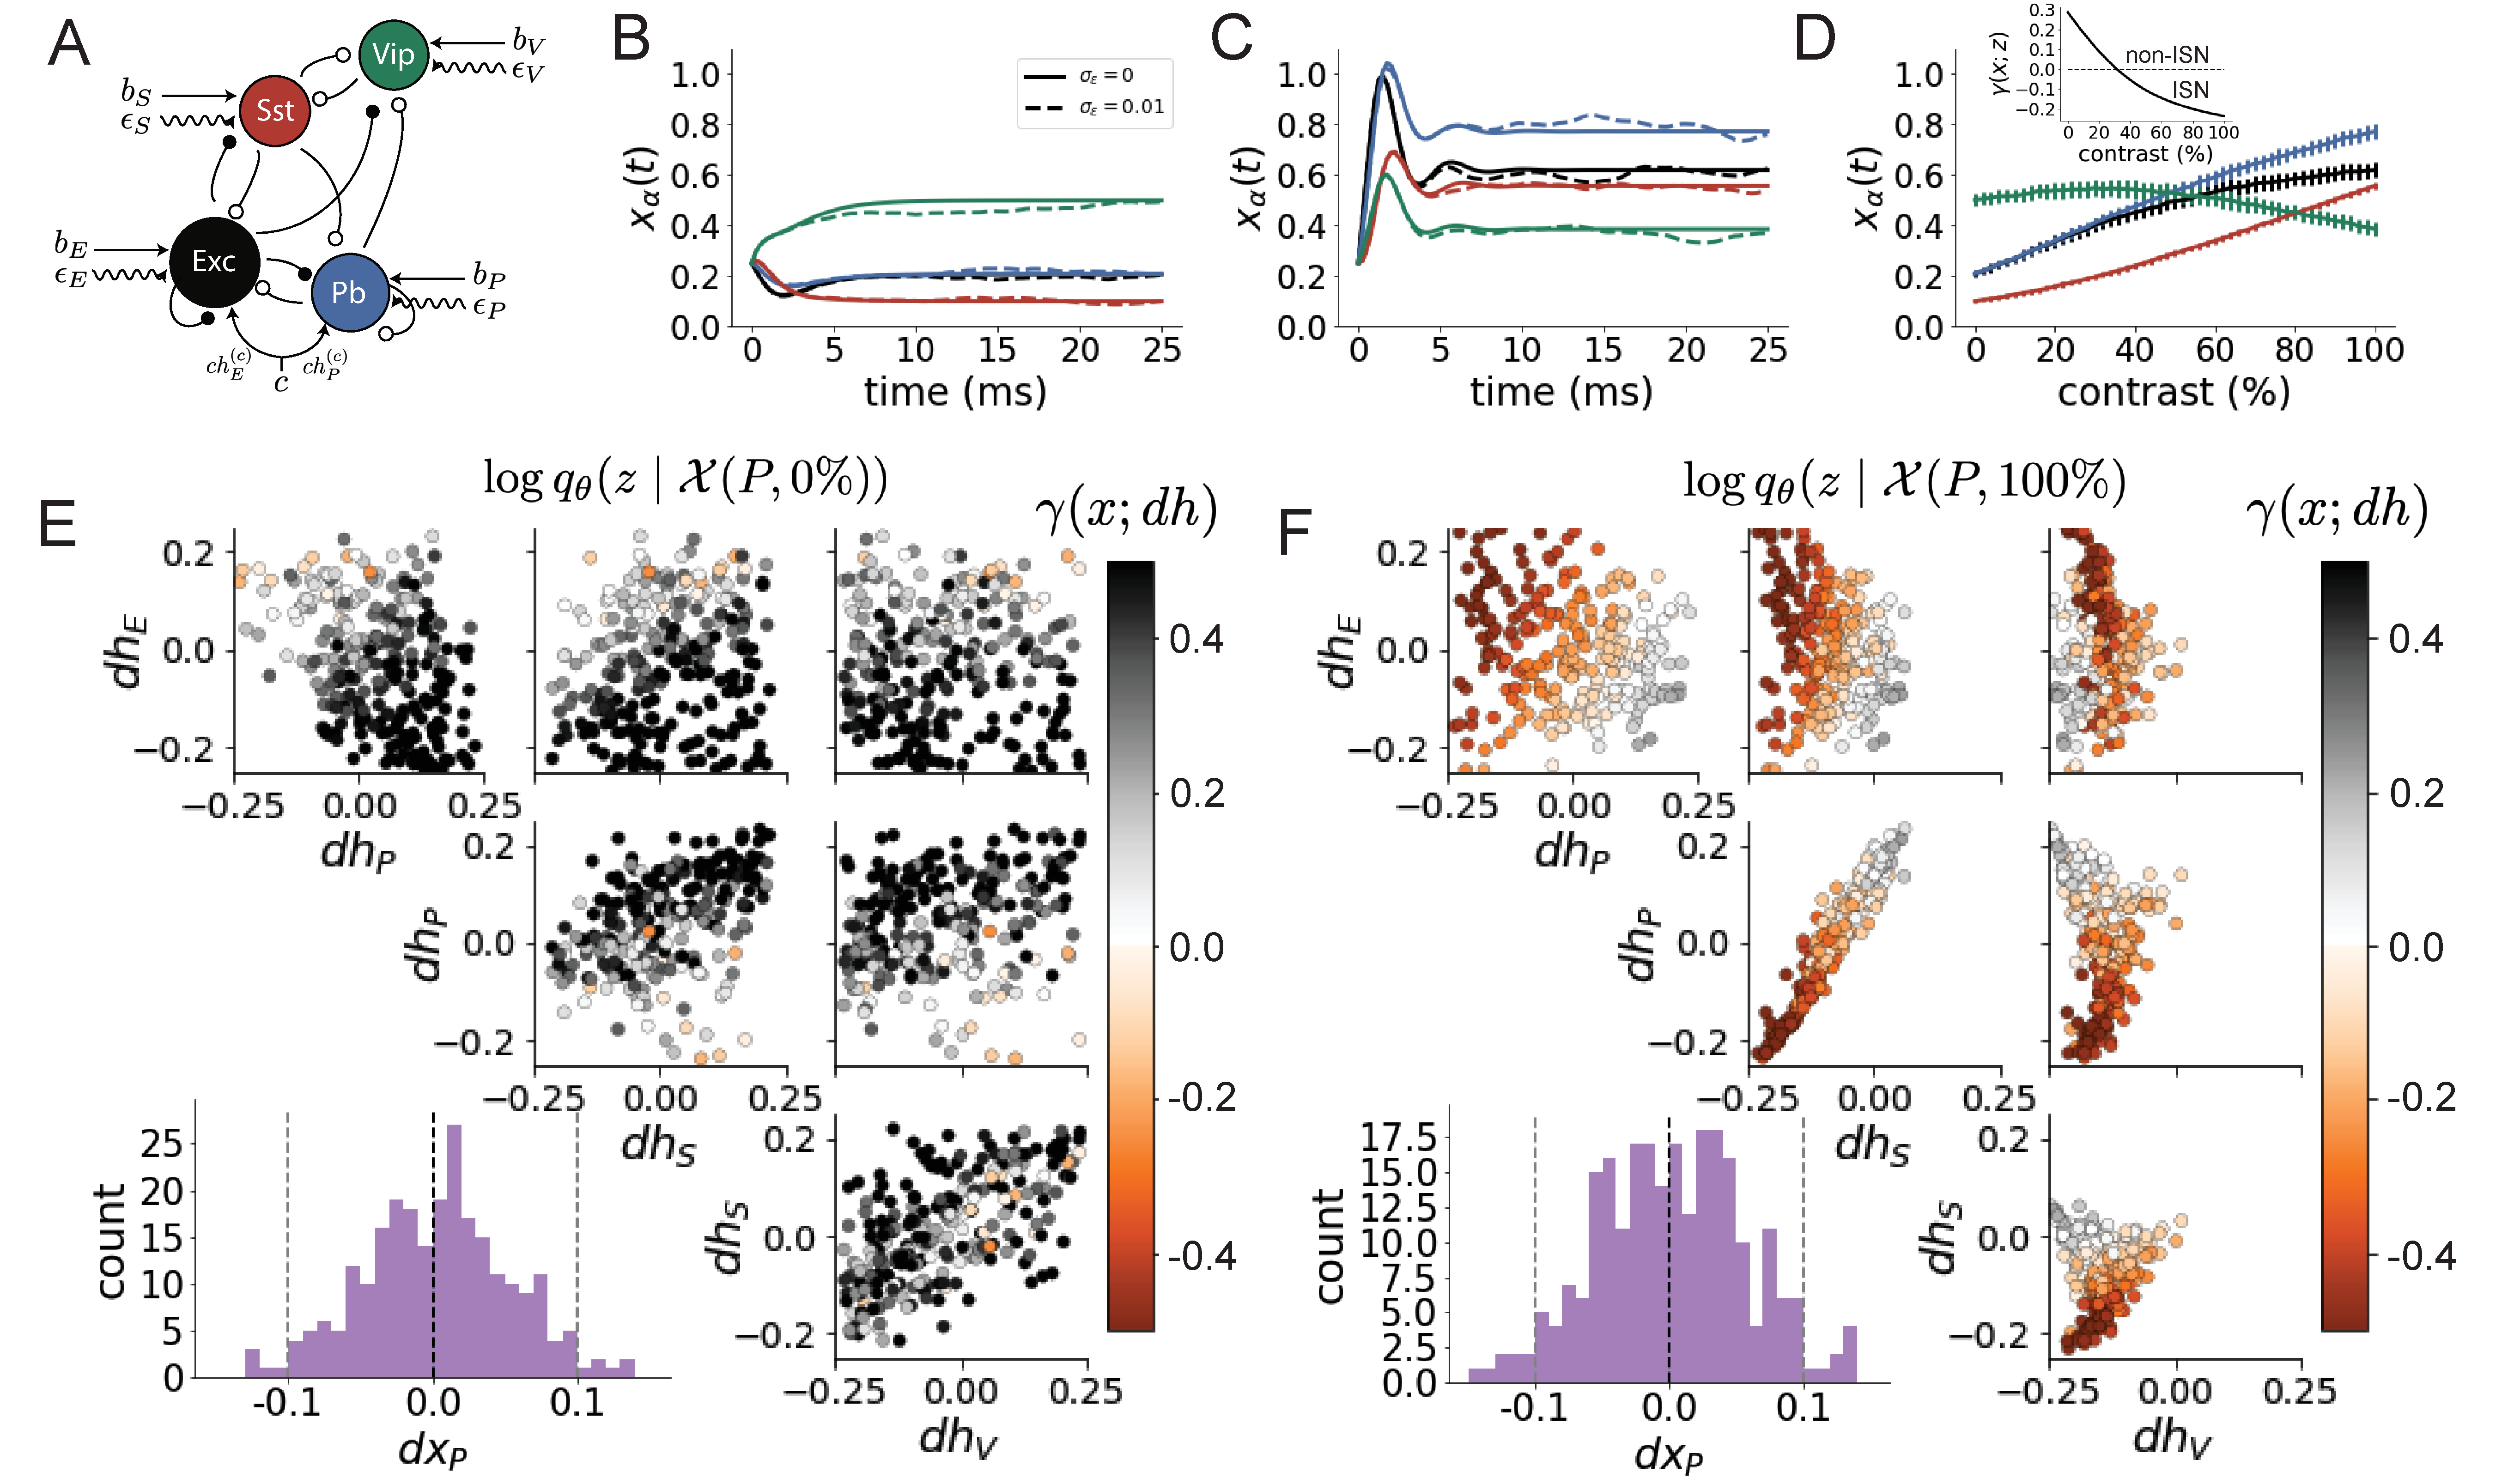
\includegraphics[scale=.18]{figs/Fig3/Fig3.pdf}
\end{center}
\end{figure}
\clearpage




\section{V1 Supplemental section}\label{methods_V1}

The dynamics are driven by the rectified and squared sum of recurrent inputs $W\mathbf{x}$, external inputs $\mathbf{h}$, and external noise:

\begin{equation}
    \tau \frac{d\mathbf{x}}{dt} = -\mathbf{x} +f_r(W\mathbf{x} + \mathbf{h} + \mathbf{\epsilon})
\end{equation}
where the input is comprised of a baseline and contrast-dependent input 
\begin{equation}
 \mathbf{h} =  \mathbf{h}_b +  c\mathbf{h}_c
\end{equation} 
$\tau = 1 \text{ms}$, $f_r(\mathbf{x}) = \left[\mathbf{x} \right]_+^2$, and $c \in \left[0, 1\right]$.

The noise is modeled as an Ornstein-Uhlenbeck process:
\begin{equation}
\tau_{\text{noise}} d\epsilon_\alpha = -\epsilon_\alpha dt + \sqrt{2\tau_{\text{noise}}}\sigma_\alpha dB
\end{equation}

where $\tau_{\text{noise}}$ is slow at 5ms, $\sigma_\alpha =  0.01 $, and $dB$ is a standard Wiener process.

We considered the stability of this stochastic stabilized supralinear network with respect to an additive differential input $d\mathbf{h}$
\begin{equation}
    \tau \frac{d\mathbf{x}}{dt} = -\mathbf{x} +f_r(W\mathbf{x} + \mathbf{h} + d\mathbf{h}+ \epsilon).
\end{equation}

We used connectivity ($W$) and input ($\mathbf{h}_b$ and $\mathbf{h}_c$) parameters fit to the deterministic model (TODO cite)

\begin{equation}
W =  \begin{bmatrix} W_{EE} & W_{EP} & W_{ES} & W_{EV} \\
W_{PE} & W_{PP} & W_{PS} & W_{PV} \\
W_{SE} & W_{SP} & W_{SS} & W_{SV} \\
W_{VE} & W_{VP} & W_{VS} & W_{VV}  \end{bmatrix} = 
 \begin{bmatrix} .785 & -.102 & -1.24 & -.306 \\
.809 & -.100 & -.620 & -.264 \\
.833 & -.000128 & -.0000483 & -.742 \\
.708 & -.306 & -.452 & -.0000605 \\
 \end{bmatrix},
\end{equation} 

\begin{equation}
\mathbf{h}_b =  \begin{bmatrix} h_{b,E} \\ h_{b,P} \\ h_{b,S} \\ h_{b,V} \end{bmatrix} =
 \begin{bmatrix} .590 \\ .504 \\ .515 \\ .670 \end{bmatrix} ,
\end{equation} 
and
\begin{equation} 
\mathbf{h}_c = \begin{bmatrix} h_{c,E} \\ h_{c,P} \\ h_{c,S} \\ h_{c,V} \end{bmatrix} = 
\begin{bmatrix} .595 \\ .396 \\ 0 \\ 0 \end{bmatrix}.
\end{equation} 

The expectation and variance in the emergent property are taken over both the posterior distribution and the stochasticity of the SSSN:
\begin{equation}
= \mathbb{E}_{\mathbf{z}}\begin{bmatrix} dx_\alpha(\mathbf{x}; \mathbf{z},c) \end{bmatrix}  = \mathbb{E}_{\mathbf{z}\sim q_\theta(\mathbf{z})} \left[ \mathbb{E}_{\mathbf{x} \sim p(\mathbf{x} \mid \mathbf{z})} \begin{bmatrix} x_\alpha(\mathbf{x}; \mathbf{z},c) - x_\alpha(\mathbf{x}; \mathbf{0},c) \end{bmatrix}\right].
\end{equation}
Thus, over the EPI posterior predictive distribution, the mean and variance of the slow fluctuations about the steady state solution are constrained to $\mu = 0$ and $\sigma^2 = 0.05^2$

This ISN coefficient of the network at a given input is calculated by simulating the system to a steady state in the absence of noise
\begin{equation}
    \gamma(\mathbf{x}; \mathbf{z}) = 1 - 2 \left[u_E \right]_+ W_{EE}
\end{equation}
where
\begin{equation}
    \mathbf{u} = W\mathbf{x} + \mathbf{h} + d\mathbf{h}.
\end{equation}

When the ISN coefficient is negative, the network is inhibition-stabilized.  
To get an idea of what distribution of parameters ($d\mathbf{h}$) we should expect from EPI, we can use ABC to obtain a set of parameters related to the emergent property.  
We compare EPI to ABC with a rejection heuristic defined by the standard deviation of the differential responses $\sigma_{ABC}$
 \begin{equation}
 f_{ABC}(dx_\alpha; \sigma_{ABC}) = |dx_\alpha| > 2\sigma_{ABC}.
 \end{equation}
 In other words, we ran ABC accepting parameters that generate differential responses within two standard deviations $\sigma_{ABC}=0.05$ of $dx_\alpha = 0$.

\begin{figure}[h]
\caption{\small Supplemental Figure: A. Top row: EPI posteriors $q_\theta(z \mid \mathcal{X}(\alpha, c)$ for neuron-type $\alpha$, 0\% contrast, $\epsilon=0.01$ visualized as samples colored by their log probability.  Bottom-left of pairplots indicate that the posterior predictive distribution obeys the emergent property constraints.  
Bottom row: Sets of parameters produced using the ABC approach.  Bottom-left of pairplots shows statistics of accepted parameters (black) and the ABC posterior predictive distribution given that set (purple).
B. Same as A at 100\% contrast.
 }\label{fig:SX1}
\begin{center}
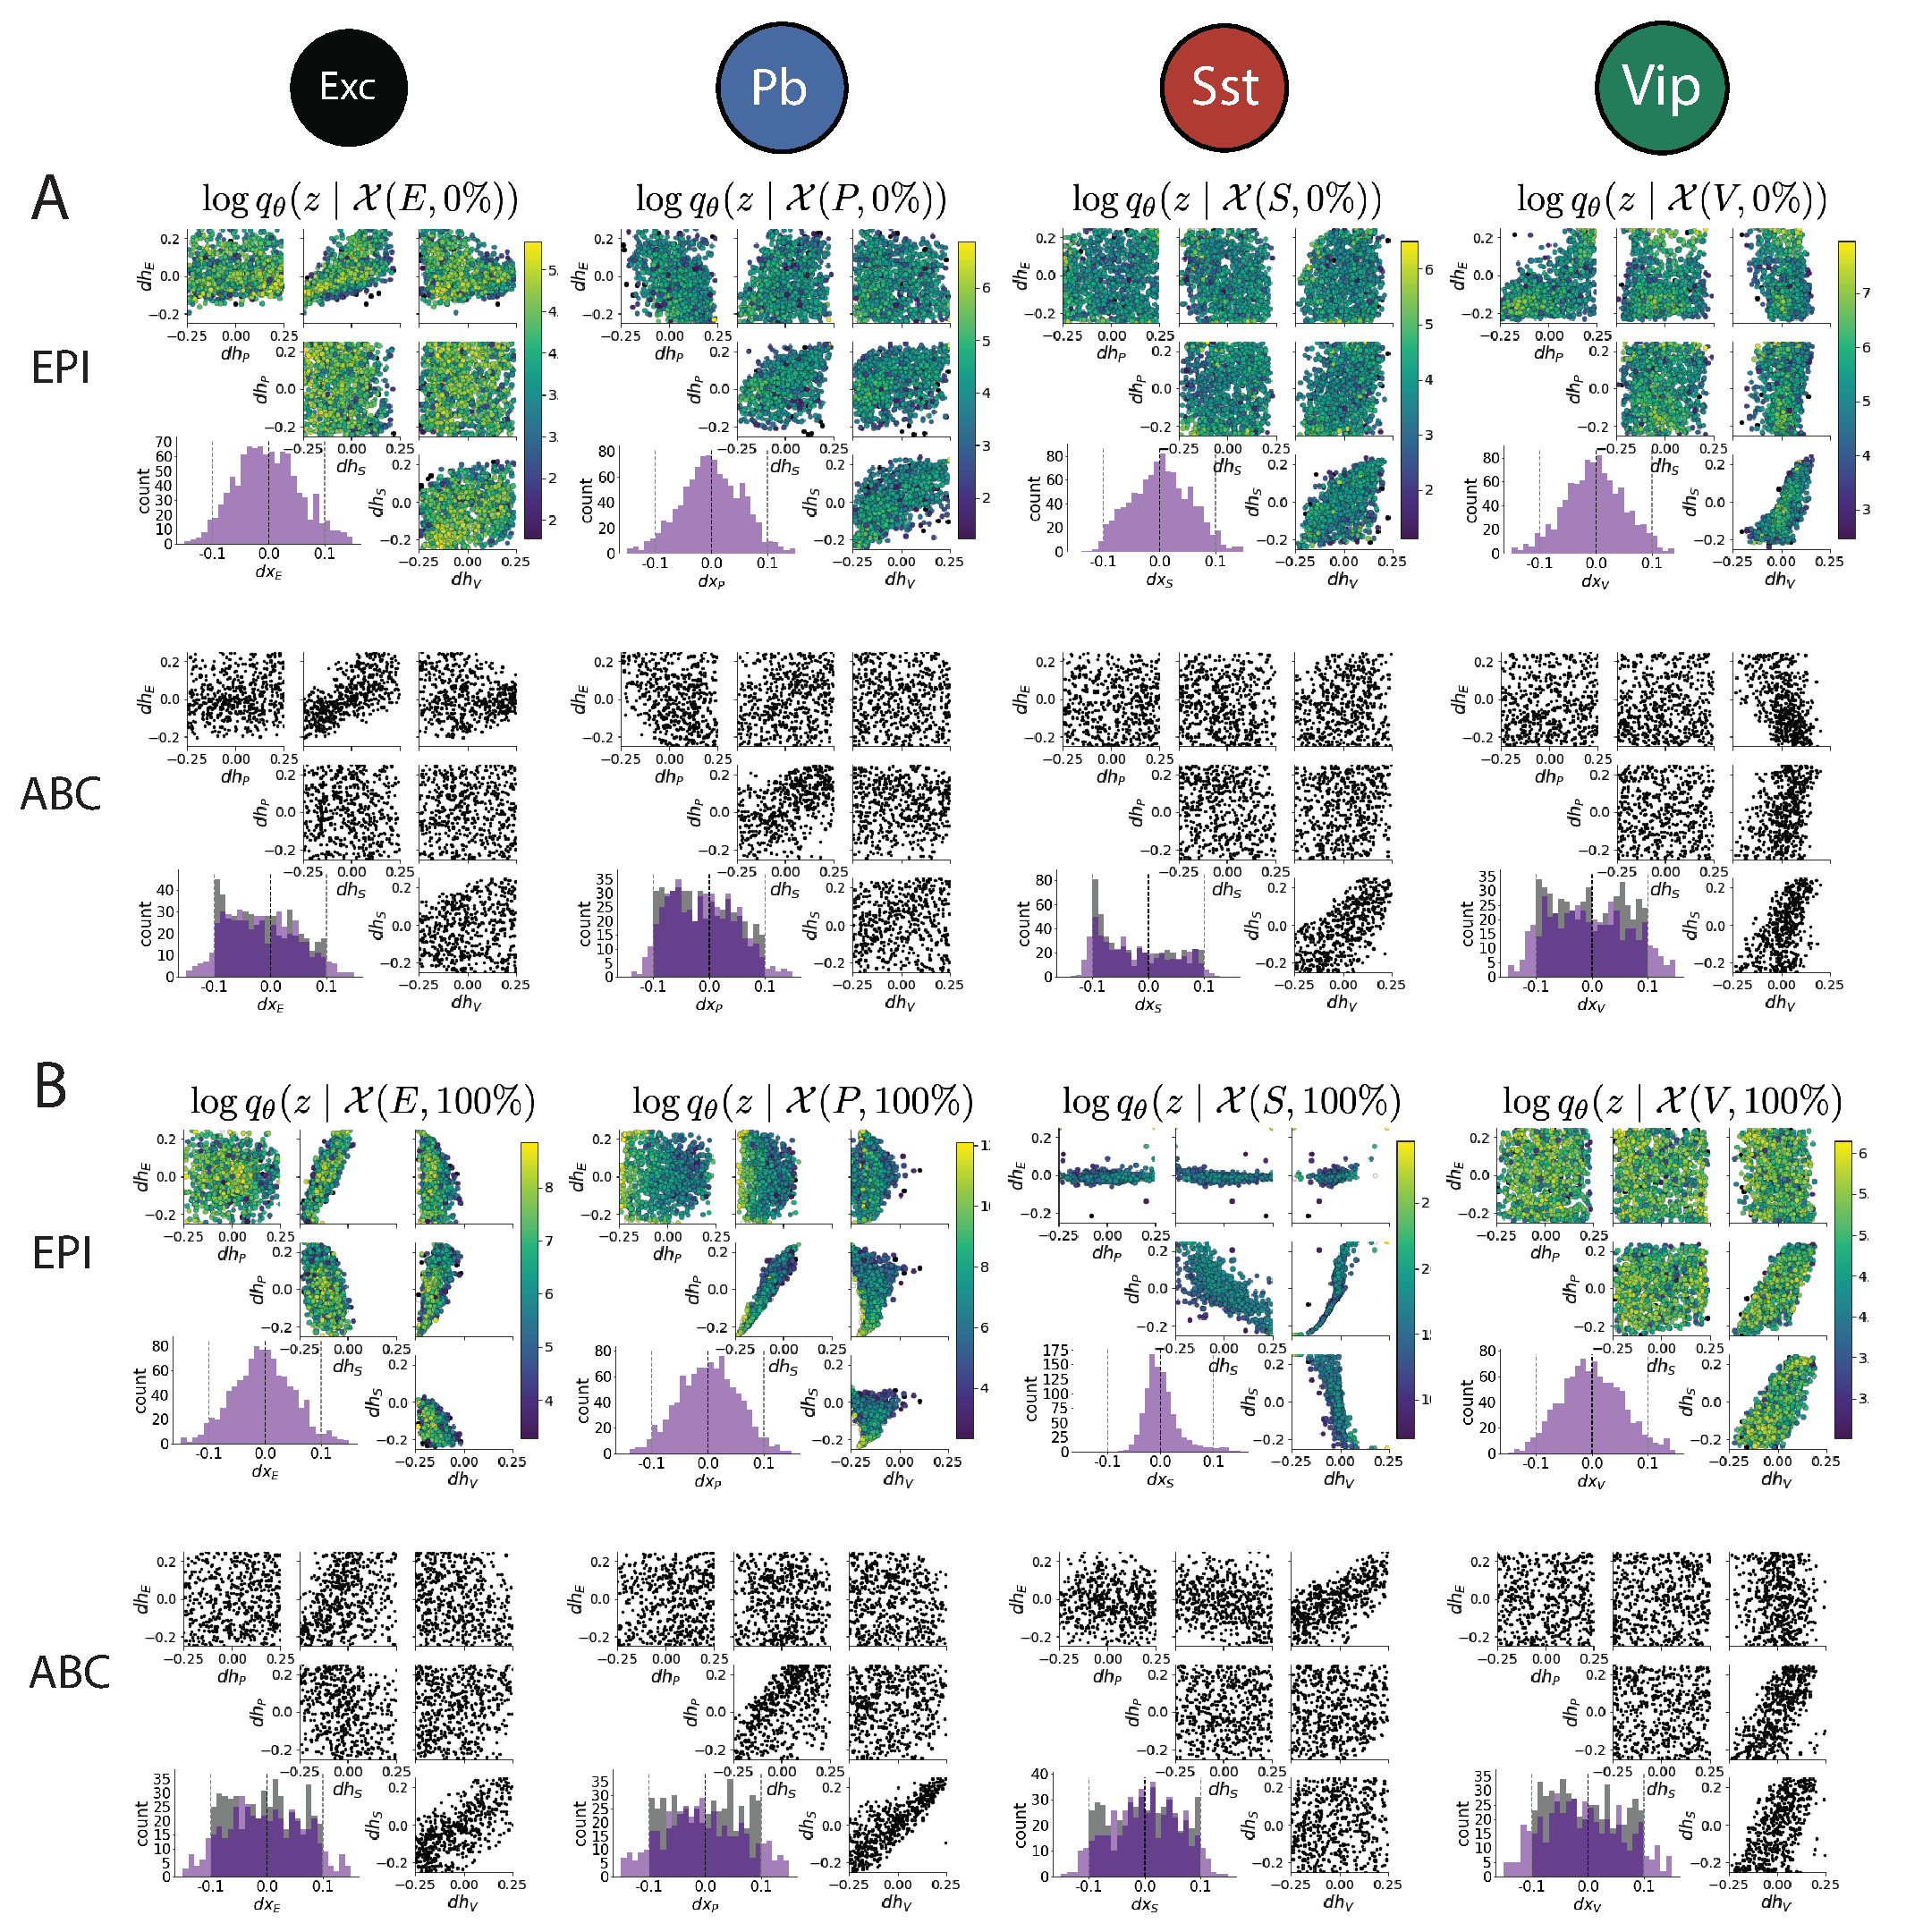
\includegraphics[scale=.5]{figs/FigSX/Fig_SX1.pdf}
\end{center}
\end{figure}

\begin{figure}[h]
\caption{\small Supplemental Figure: Same as Figure 2 (will be supp fig) with $\sigma_{\epsilon} = 0.001$.
 }\label{fig:SX2}
\begin{center}
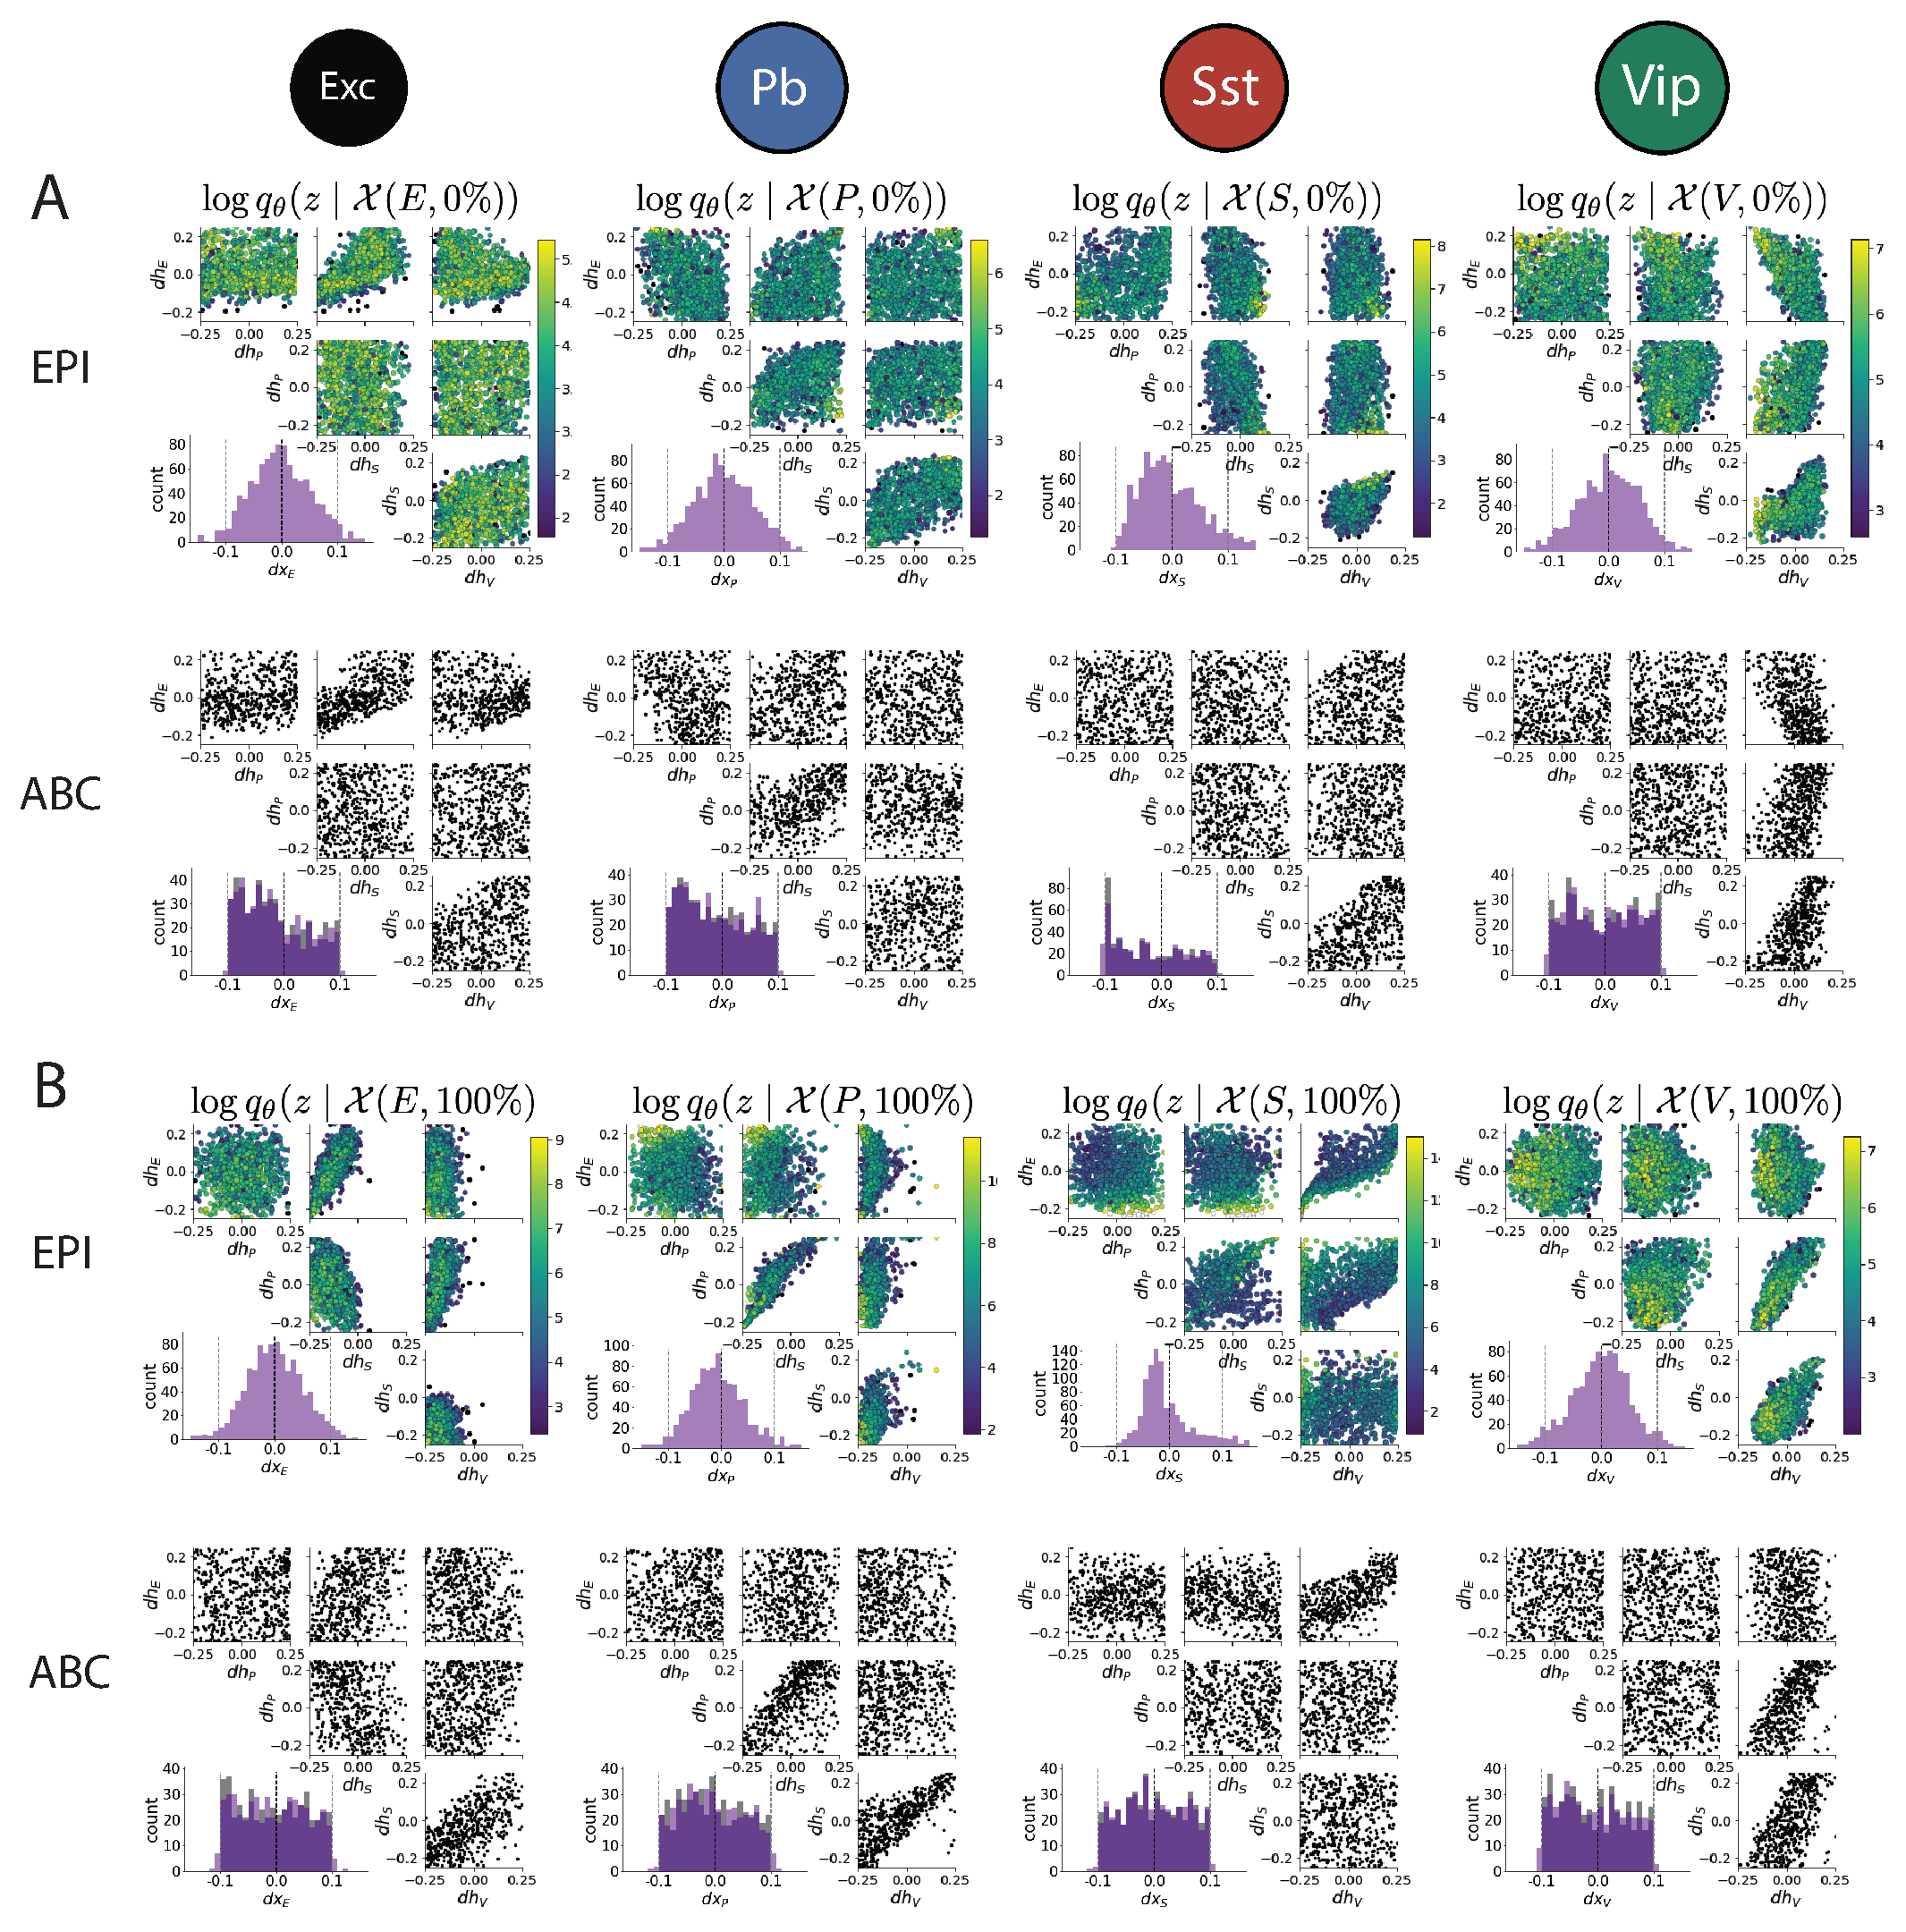
\includegraphics[scale=.5]{figs/FigSX/Fig_SX2.pdf}
\end{center}
\end{figure}


\bibliography{epi}
\bibliographystyle{unsrt}

\end{document}
